% Compile: pdflatex slides.tex
% Target length: 15 min talk -- ~15-17 content slides + title + thanks.
\documentclass[aspectratio=169,12pt,xcolor={table}]{beamer}
\usetheme{metropolis}   % if unavailable, fall back to \usetheme{default}
\usepackage{graphicx}
\usepackage{booktabs}
\usepackage{amsmath}
\usepackage{colortbl}
\usepackage{array}

\definecolor{accent}{HTML}{1F6FEB}
\setbeamercolor{progress bar}{fg=accent}
\setbeamercolor{title separator}{fg=accent}
\setbeamercolor{frametitle}{bg=accent,fg=white}

\title{Deep Learning-Based Land Cover Segmentation\\from Satellite Imagery}
\subtitle{Architectures, Transfer Learning, and Loss Functions}
\author{Rongxuan Zhang}
\institute{Northeastern University\\EECE 7370 Advanced Computer Vision}
\date{April 18, 2026}

\begin{document}

% ============================================================================
\begin{frame}
  \titlepage
\end{frame}

% ============================================================================
\section{Motivation}

\begin{frame}{Why land-cover segmentation?}
  \begin{columns}[T]
  \column{0.55\textwidth}
  \textbf{Applications}
  \begin{itemize}
    \item Urban planning (city growth, land use)
    \item Precision agriculture (crop distribution)
    \item Ecological monitoring (deforestation)
    \item Climate and disaster response
  \end{itemize}

  \vspace{0.8em}
  \textbf{Task.} Given a $2448\times2448$ RGB satellite image, predict
  per-pixel class from \{Urban, Agriculture, Rangeland, Forest, Water,
  Barren, Unknown\}.

  \column{0.43\textwidth}
  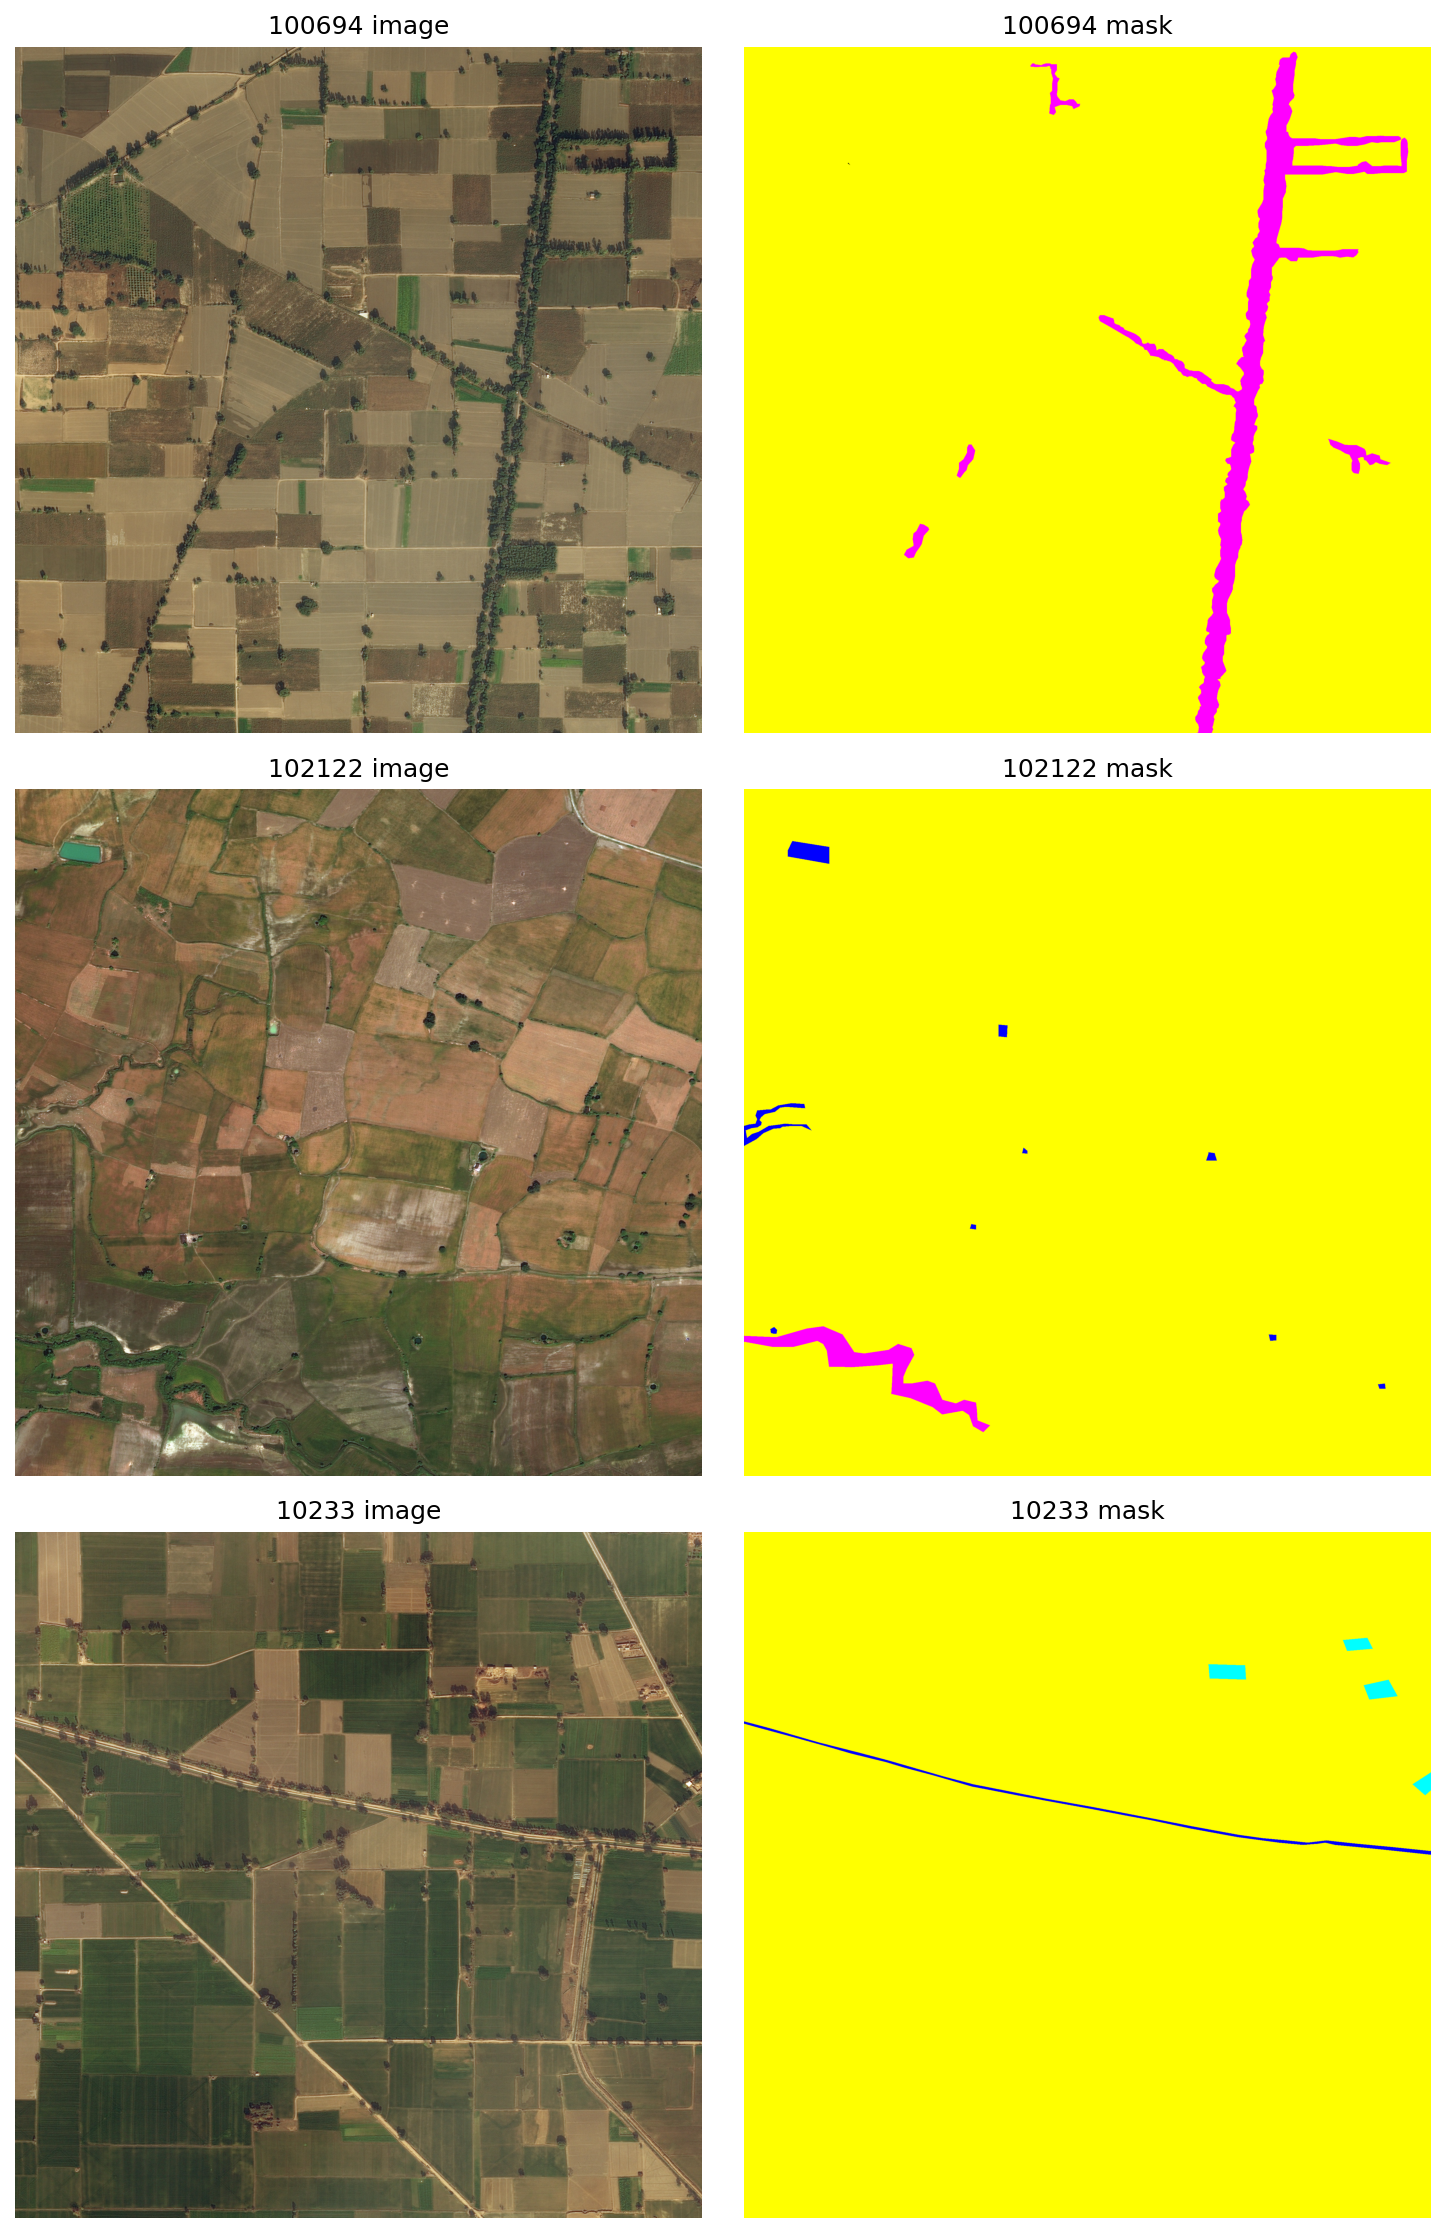
\includegraphics[width=\linewidth]{figs/samples.png}
  \end{columns}
\end{frame}

\begin{frame}{Three technical challenges}
  \begin{enumerate}
    \item \textbf{Resolution:} $2448^2$ images exceed GPU memory at any
          reasonable batch size.
    \item \textbf{Class imbalance:} Water + Barren = $<$7\% of pixels;
          cross-entropy gradients are swamped by the 55\% Agriculture class.
    \item \textbf{Cost vs.\ accuracy:} many architecture/loss choices; which
          knobs actually matter?
  \end{enumerate}

  \vspace{0.8em}
  \begin{block}{Research questions}
  (i) How much does ImageNet pre-training help?\\
  (ii) Do deeper decoders beat U-Net at this resolution?\\
  (iii) Which loss best recovers minority classes?
  \end{block}
\end{frame}

% ============================================================================
\section{Dataset \& Pipeline}

\begin{frame}{DeepGlobe Land Cover Classification}
  \begin{itemize}
    \item \textbf{803} manually-annotated $2448^2$ RGB images, 7 classes
    \item Split \textbf{at the image level} (no tile leakage):
          562 train / 121 val / 120 test
    \item Unknown class (6) treated as \texttt{ignore\_index}---consistent
          with the official DeepGlobe protocol
  \end{itemize}

  \vspace{0.6em}
  \begin{center}
  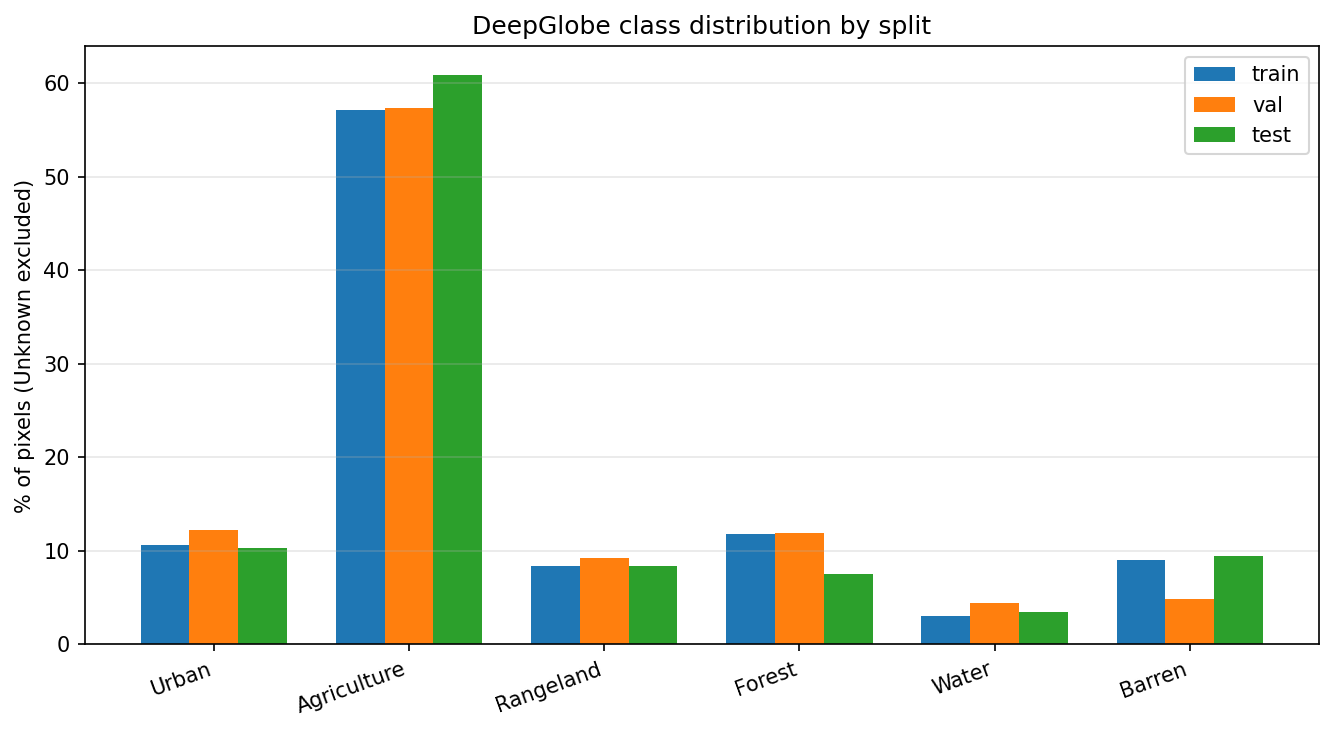
\includegraphics[width=0.85\linewidth]{figs/class_dist.png}
  \end{center}
\end{frame}

\begin{frame}{Tiling pipeline}
  \begin{columns}
  \column{0.52\textwidth}
  \textbf{Training.} Each $2448^2$ image $\rightarrow$ $3\times3$ grid of
  $816\times816$ tiles $\rightarrow$ 5058 train tiles total.

  \vspace{0.4em}
  \textbf{Padding.} $816 \bmod 32 = 16$; reflect-pad to $832^2$ to satisfy
  5-stage encoder constraint. Padded mask = ignore.

  \vspace{0.4em}
  \textbf{Inference.} Sliding window ($816$ tile + 64 overlap) over
  full $2448^2$ image; softmax probabilities averaged in overlapping
  regions before argmax.

  \column{0.45\textwidth}
  \vspace{-0.5em}
  \small
  \begin{tabular}{c|c|c}
    \multicolumn{3}{c}{$2448 \times 2448$}\\\hline
     t1 & t2 & t3 \\\hline
     t4 & t5 & t6 \\\hline
     t7 & t8 & t9 \\
  \end{tabular}

  \vspace{1em}
  \footnotesize
  \textbf{Why tile?} Preserves native resolution (vs.\ resizing).\\
  \textbf{Why pad?} smp encoders need H,W divisible by 32.\\
  \textbf{Why overlap?} Reduces boundary artifacts at stitch.
  \end{columns}
\end{frame}

% ============================================================================
\section{Method}

\begin{frame}{Experimental grid}
  \textbf{Phase 4} -- architecture, fixed loss (CE), 6 runs:
  \small
  \begin{itemize}
    \item Vanilla U-Net (scratch) \hspace{1em}\textit{Ronneberger-style baseline}
    \item U-Net + ResNet34 (scratch) \hspace{1em}\textit{isolates arch effect}
    \item U-Net + ResNet34 (ImageNet) \hspace{1em}\textit{isolates transfer}
    \item DeepLabV3+ + ResNet50 (ImageNet)
    \item DeepLabV3+ + ResNet101 (ImageNet)
    \item Attention U-Net + ResNet34 + SCSE (ImageNet)
  \end{itemize}

  \vspace{0.4em}
  \textbf{Phase 5} -- loss, fixed arch (Phase 4 winner = DeepLabV3+-R50), 4 runs:
  \begin{itemize}
    \item Cross-Entropy (baseline)
    \item Dice
    \item Focal ($\alpha{=}0.25,\gamma{=}2$)
    \item Combined ($0.5 \cdot \text{CE} + 0.5 \cdot \text{Dice}$)
  \end{itemize}

  \vspace{0.4em}
  \textbf{Phase 6} -- all 9 checkpoints evaluated at full $2448^2$ resolution.
\end{frame}

\begin{frame}{Training setup}
  \begin{columns}[T]
  \column{0.5\textwidth}
  \textbf{Shared hyperparameters}
  \begin{itemize}
    \item AdamW, $\text{lr}=10^{-4}$, wd $10^{-4}$
    \item Cosine annealing, 50 epochs
    \item Early stopping, patience 10
    \item Mixed precision (fp16)
    \item Batch size 8 (4 for R101 OOM)
  \end{itemize}

  \column{0.5\textwidth}
  \textbf{Augmentations} (Albumentations)
  \begin{itemize}
    \item H/V flip, 90$^\circ$ rotation
    \item $\pm15^\circ$ affine
    \item Brightness/contrast jitter
    \item Gaussian noise
  \end{itemize}

  \vspace{0.5em}
  \textbf{Compute}
  \begin{itemize}
    \item Colab Pro+, 1$\times$ A100 40GB
    \item $\sim$15 GPU-hours total
    \item W\&B + Drive checkpointing
  \end{itemize}
  \end{columns}
\end{frame}

% ============================================================================
\section{Results}

\begin{frame}{Training dynamics (Phase 4)}
  \centering
  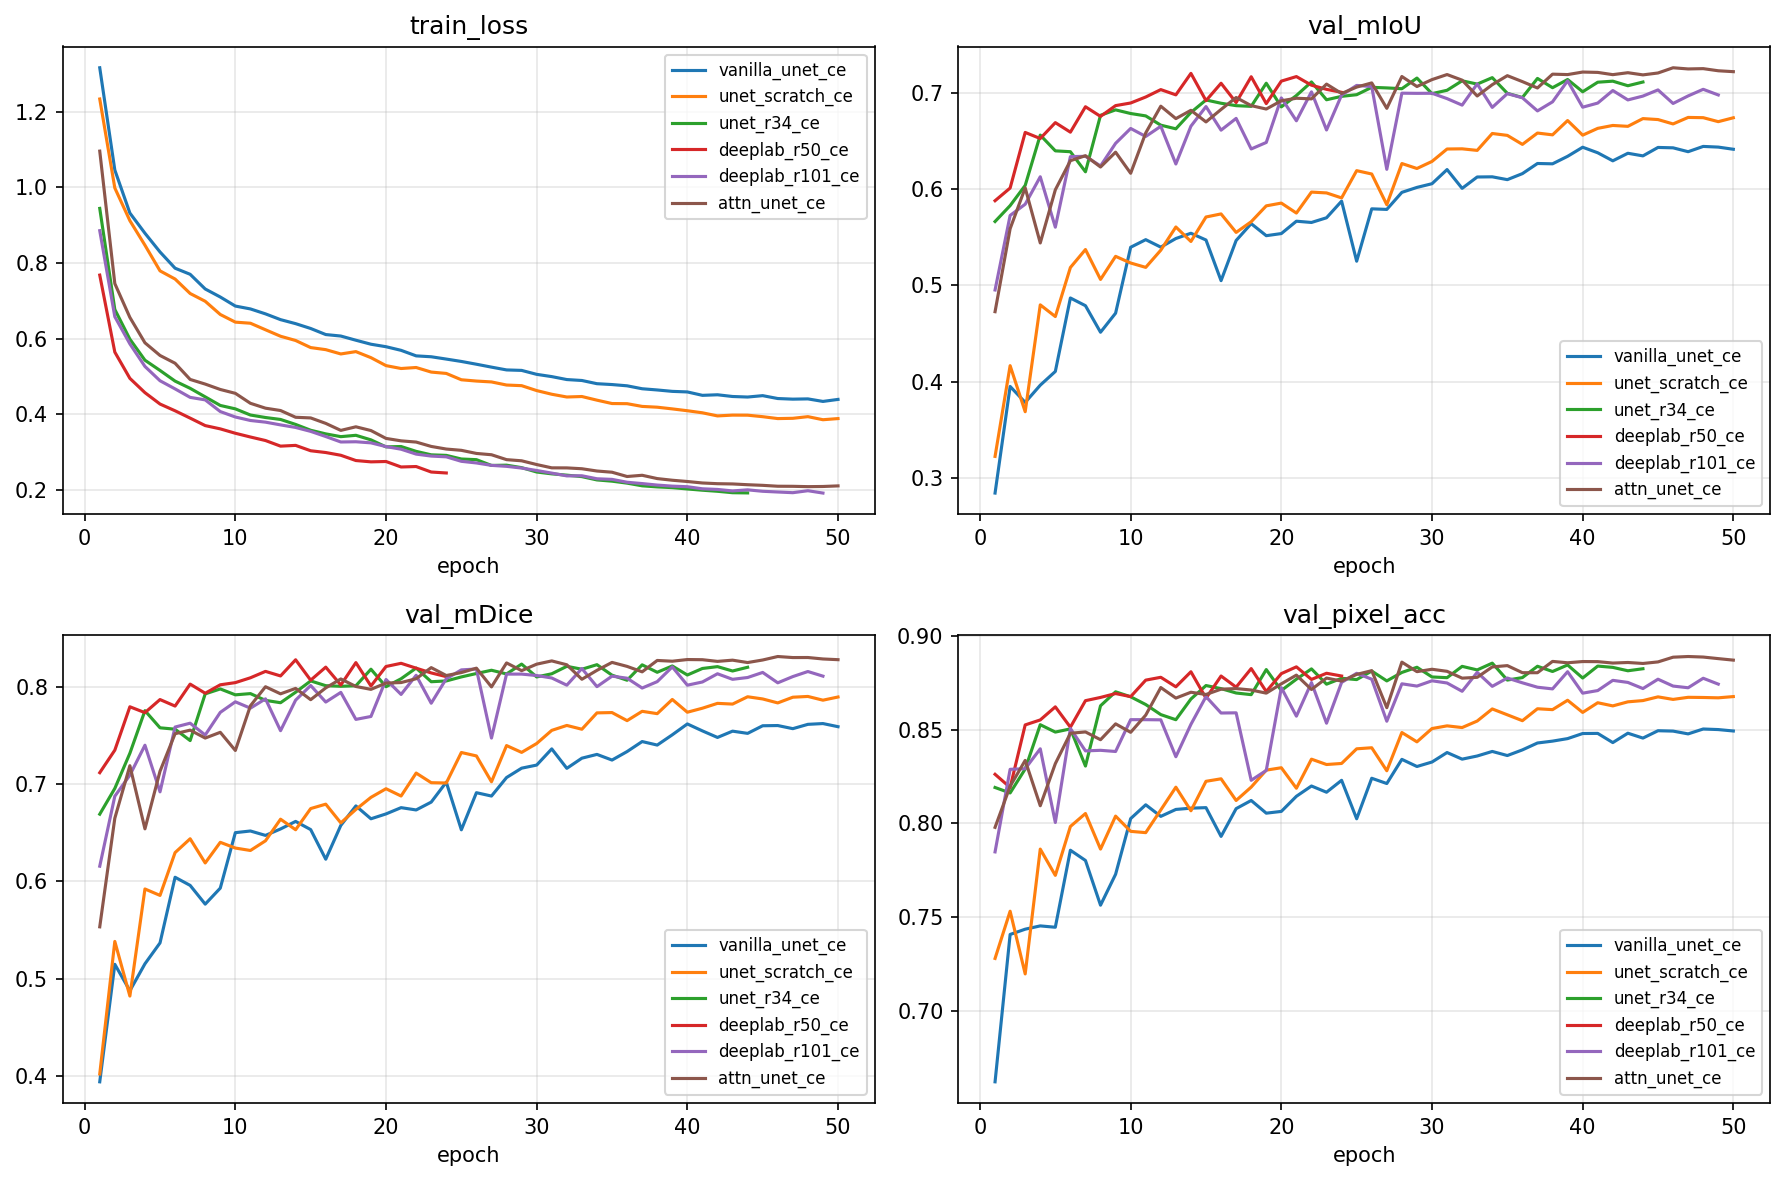
\includegraphics[width=0.95\linewidth]{figs/curves_archs.png}

  \vspace{0.5em}
  \small
  Pre-trained runs cross 0.6 mIoU in $\le$3 epochs; scratch runs need 12--20.
\end{frame}

\begin{frame}{Phase 4: architecture ranking}
  \small
  \begin{tabular}{l c c c c c}
  \toprule
  Model & Params (M) & Train (h) & Val mIoU & Test mIoU & GPU peak \\
  \midrule
  Vanilla U-Net (scratch)         & 31.04 & 3.53 & 0.6442 & 0.6402 & -- \\
  U-Net R34 (scratch)             & 24.44 & 2.00 & 0.6743 & 0.6750 & -- \\
  U-Net R34 (ImageNet)            & 24.44 & 1.76 & 0.7156 & 0.7093 & -- \\
  DeepLabV3+ R50 (ImageNet)       & 26.68 & \textbf{0.97} & 0.7201 & 0.6963 & 8.0 GB \\
  DeepLabV3+ R101 (ImageNet)      & 45.67 & 2.32 & 0.7124 & 0.7178 & 5.6 GB \\
  \rowcolor{accent!15}
  Attention U-Net R34 (ImageNet)  & 24.55 & 2.20 & \textbf{0.7259} & \textbf{0.7316} & 7.0 GB \\
  \bottomrule
  \end{tabular}

  \vspace{0.8em}
  \textbf{Three observations:}
  \begin{itemize}
    \item Transfer learning: +7.1\% mIoU (scratch $\rightarrow$ pre-trained)
    \item Architecture: $\le +1.5\%$ for any decoder swap
    \item R101 $<$ R50 ($-0.08$) despite 71\% more params $\rightarrow$
          overfitting on 5058 training tiles
  \end{itemize}
\end{frame}

\begin{frame}{Finding 1: Pre-training is the largest single-variable lever}
  \centering
  \small
  \begin{tabular}{l c c}
  \toprule
  Configuration (each row changes only one factor) & Val mIoU & $\Delta$ \\
  \midrule
    Vanilla U-Net (scratch, Ronneberger)                    & 0.6442 & --- \\
    $\rightarrow$ swap decoder: U-Net + ResNet34 (scratch)  & 0.6743 & $+0.030$ \\
    $\rightarrow$ \textbf{add ImageNet pretraining} (same arch.)    & \textbf{0.7156} & \textbf{$+0.041$} \\
    $\rightarrow$ swap decoder: DeepLabV3+-R50              & 0.7201 & $+0.004$ \\
    $\rightarrow$ swap decoder: Attention U-Net (SCSE)      & 0.7259 & $+0.006$ \\
  \bottomrule
  \end{tabular}

  \vspace{0.8em}
  \small
  \textbf{Isolated effect of pre-training (row 3 vs row 2):} \textbf{$+4.1$ mIoU}\\
  \textbf{Isolated effect of any single decoder change:} $\le +1.0$
\end{frame}

\begin{frame}{Finding 2: Combined loss rescues minority classes}
  \small
  \begin{tabular}{l c c c c}
  \toprule
  Loss (on DeepLabV3+-R50) & Val mIoU & Test mIoU & Barren IoU & Rangeland IoU \\
  \midrule
  Cross-Entropy (baseline) & 0.7201 & 0.6963 & 0.656 & 0.415 \\
  Dice                     & 0.7314 & 0.7214 & 0.666 & 0.443 \\
  Focal                    & 0.7286 & 0.7217 & 0.667 & 0.451 \\
  \rowcolor{accent!15}
  Combined (CE + Dice)     & \textbf{0.7382} & \textbf{0.7332} & \textbf{0.676} & \textbf{0.454} \\
  \bottomrule
  \end{tabular}

  \vspace{0.8em}
  \begin{columns}
  \column{0.58\textwidth}
  \small
  \textbf{Loss-only effect (fixed arch.\ = DeepLabV3+-R50):}
  \begin{itemize}
    \item Test mIoU: $0.696 \to 0.733$ \hspace{0.2em}(\textbf{+3.7 pts})
    \item Barren test IoU: $0.656 \to 0.676$ \hspace{0.2em}(\textbf{+2.0 pts})
    \item All three rebalanced losses $>$ CE on Barren, Water, Rangeland
  \end{itemize}
  \vspace{0.3em}
  \textbf{Stacked with arch.\ change} (vs.\ Vanilla U-Net + CE):
  \begin{itemize}
    \item Barren: $0.571 \to 0.676$ \hspace{0.2em}(\textbf{+10.5 pts total})
  \end{itemize}
  \column{0.38\textwidth}
  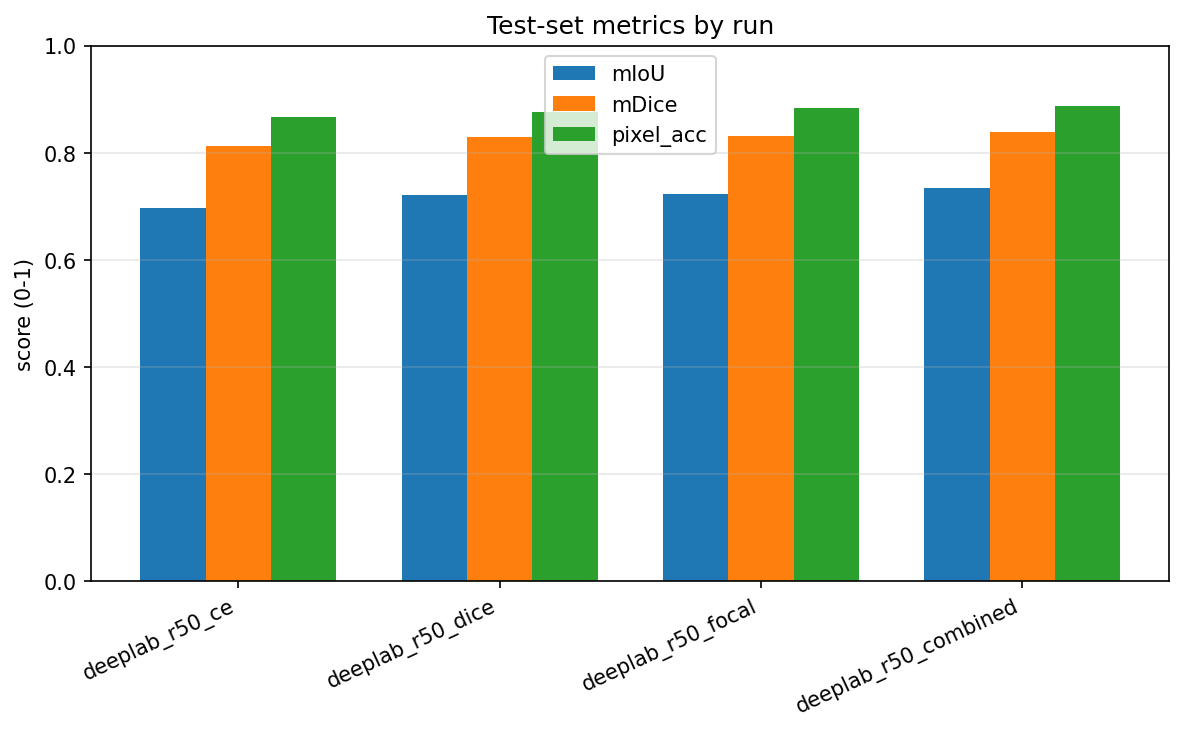
\includegraphics[width=\linewidth]{figs/losses_metrics.png}
  \end{columns}
\end{frame}

\begin{frame}{Finding 3: Deeper $\neq$ Pareto-optimal}
  \begin{columns}
  \column{0.46\textwidth}
  \textbf{DeepLabV3+ R50 vs.\ R101}
  \vspace{0.4em}
  \small
  \begin{tabular}{l c c}
  \toprule
                    & R50   & R101  \\
  \midrule
  Params (M)        & 26.68 & 45.67 \\
  GPU peak (GB)     & 8.0   & 5.6   \\
  Train time (h)    & \textbf{0.97} & 2.32 \\
  Infer (ms/img)    & \textbf{838} & 891 \\
  Val mIoU          & \textbf{0.7201} & 0.7124 \\
  Test mIoU         & 0.6963 & \textbf{0.7178} \\
  \bottomrule
  \end{tabular}

  \column{0.54\textwidth}
  \textbf{Mixed result}
  \begin{itemize}
    \item R101 wins test mIoU by $+0.022$ but loses val by $-0.008$
    \item $71\%$ more params, $2.4\times$ train time, $\sim 6\%$ slower
          inference
    \item bs=4 (R101) vs bs=8 (R50): R101 had noisier gradients during
          training
  \end{itemize}

  \vspace{0.4em}
  \textbf{Takeaway.} For DeepGlobe's 5058-tile training set, the
  ResNet50 encoder offers a better \emph{cost / accuracy} ratio. A
  small test-set gain from R101 does not justify its 2.4$\times$ cost.
  \end{columns}
\end{frame}

\begin{frame}{Confusion matrices}
  \begin{columns}
  \column{0.49\textwidth}
  \centering
  \scriptsize Attention U-Net + CE\\
  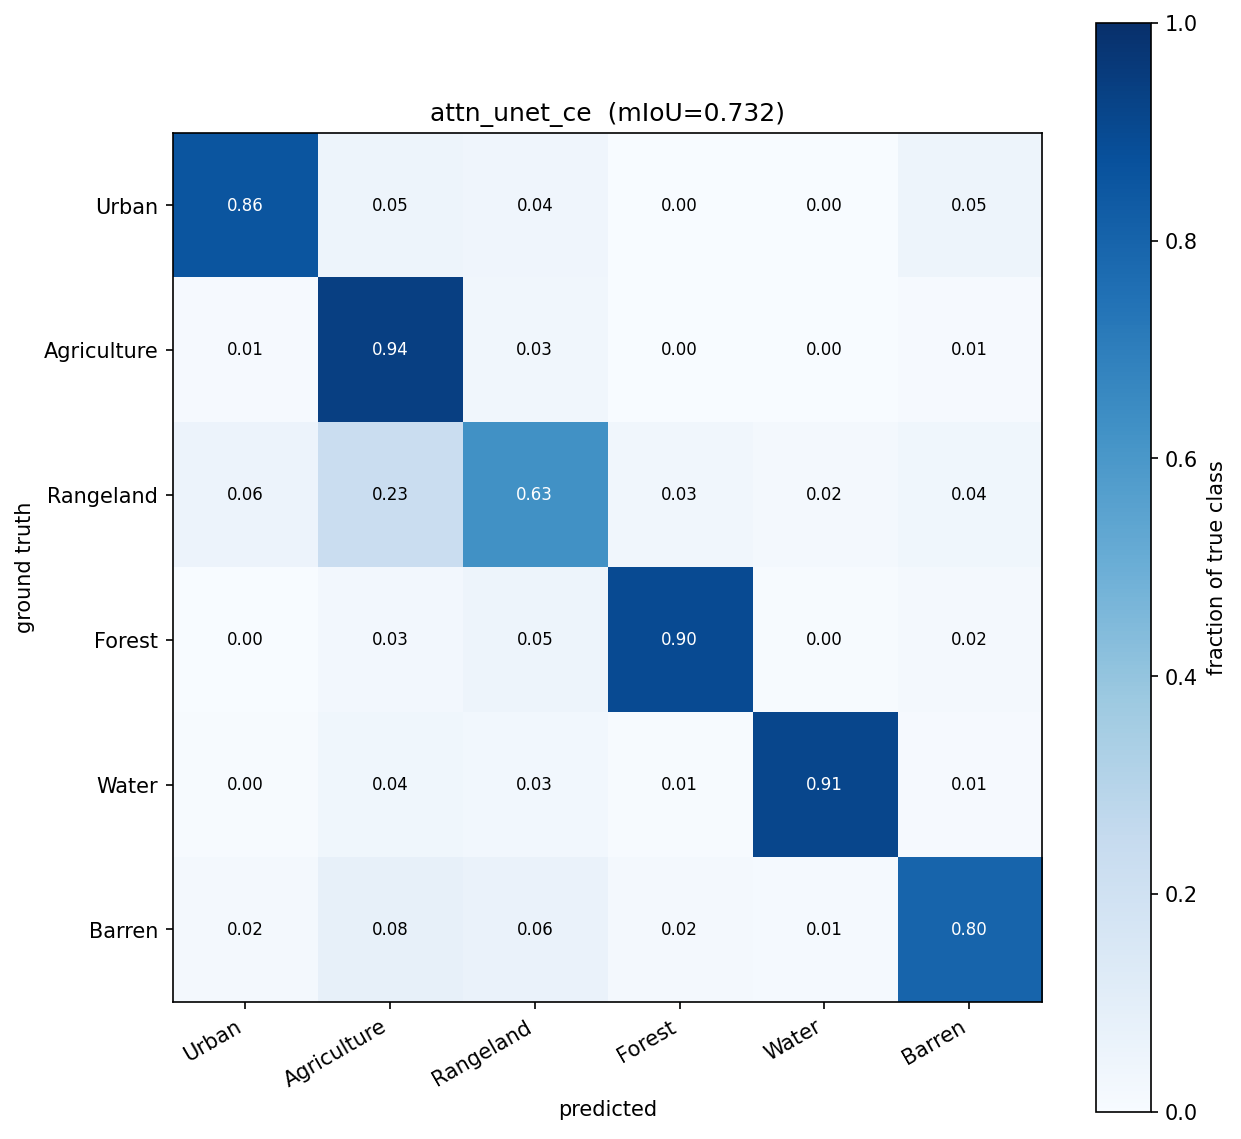
\includegraphics[width=\linewidth]{figs/cm_attn_unet_ce.png}
  \column{0.49\textwidth}
  \centering
  \scriptsize DeepLabV3+-R50 + Combined (winner)\\
  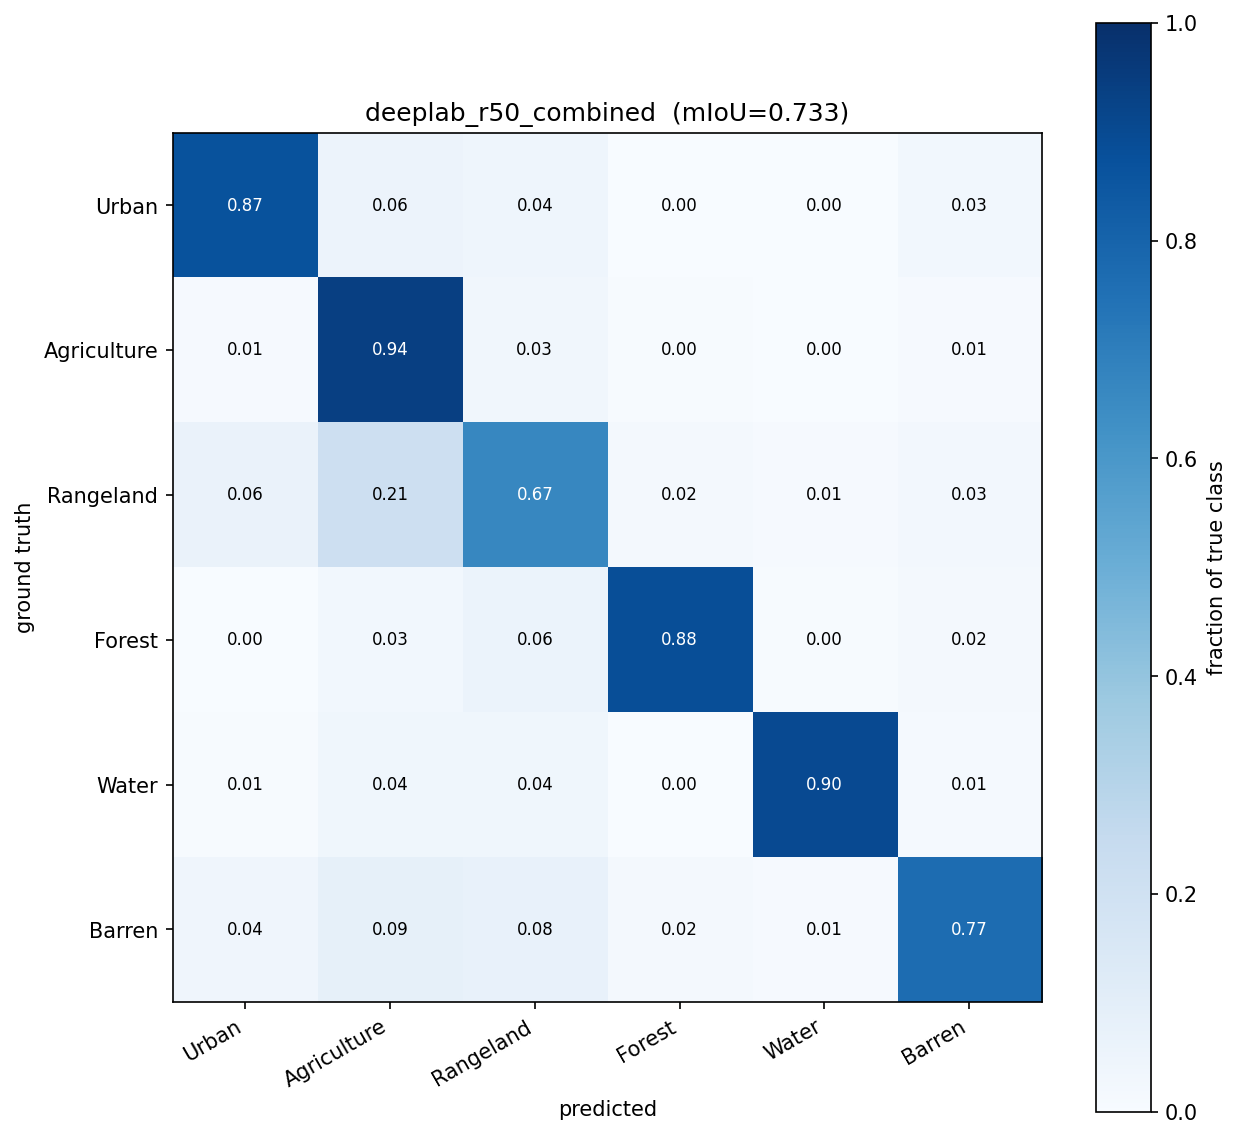
\includegraphics[width=\linewidth]{figs/cm_deeplab_r50_combined.png}
  \end{columns}

  \vspace{0.4em}
  \footnotesize
  Shared failure mode: Rangeland $\leftrightarrow$ Forest/Agriculture
  confusion---these classes have similar spectral \& textural signatures.
\end{frame}

\begin{frame}{Qualitative comparison}
  \centering
  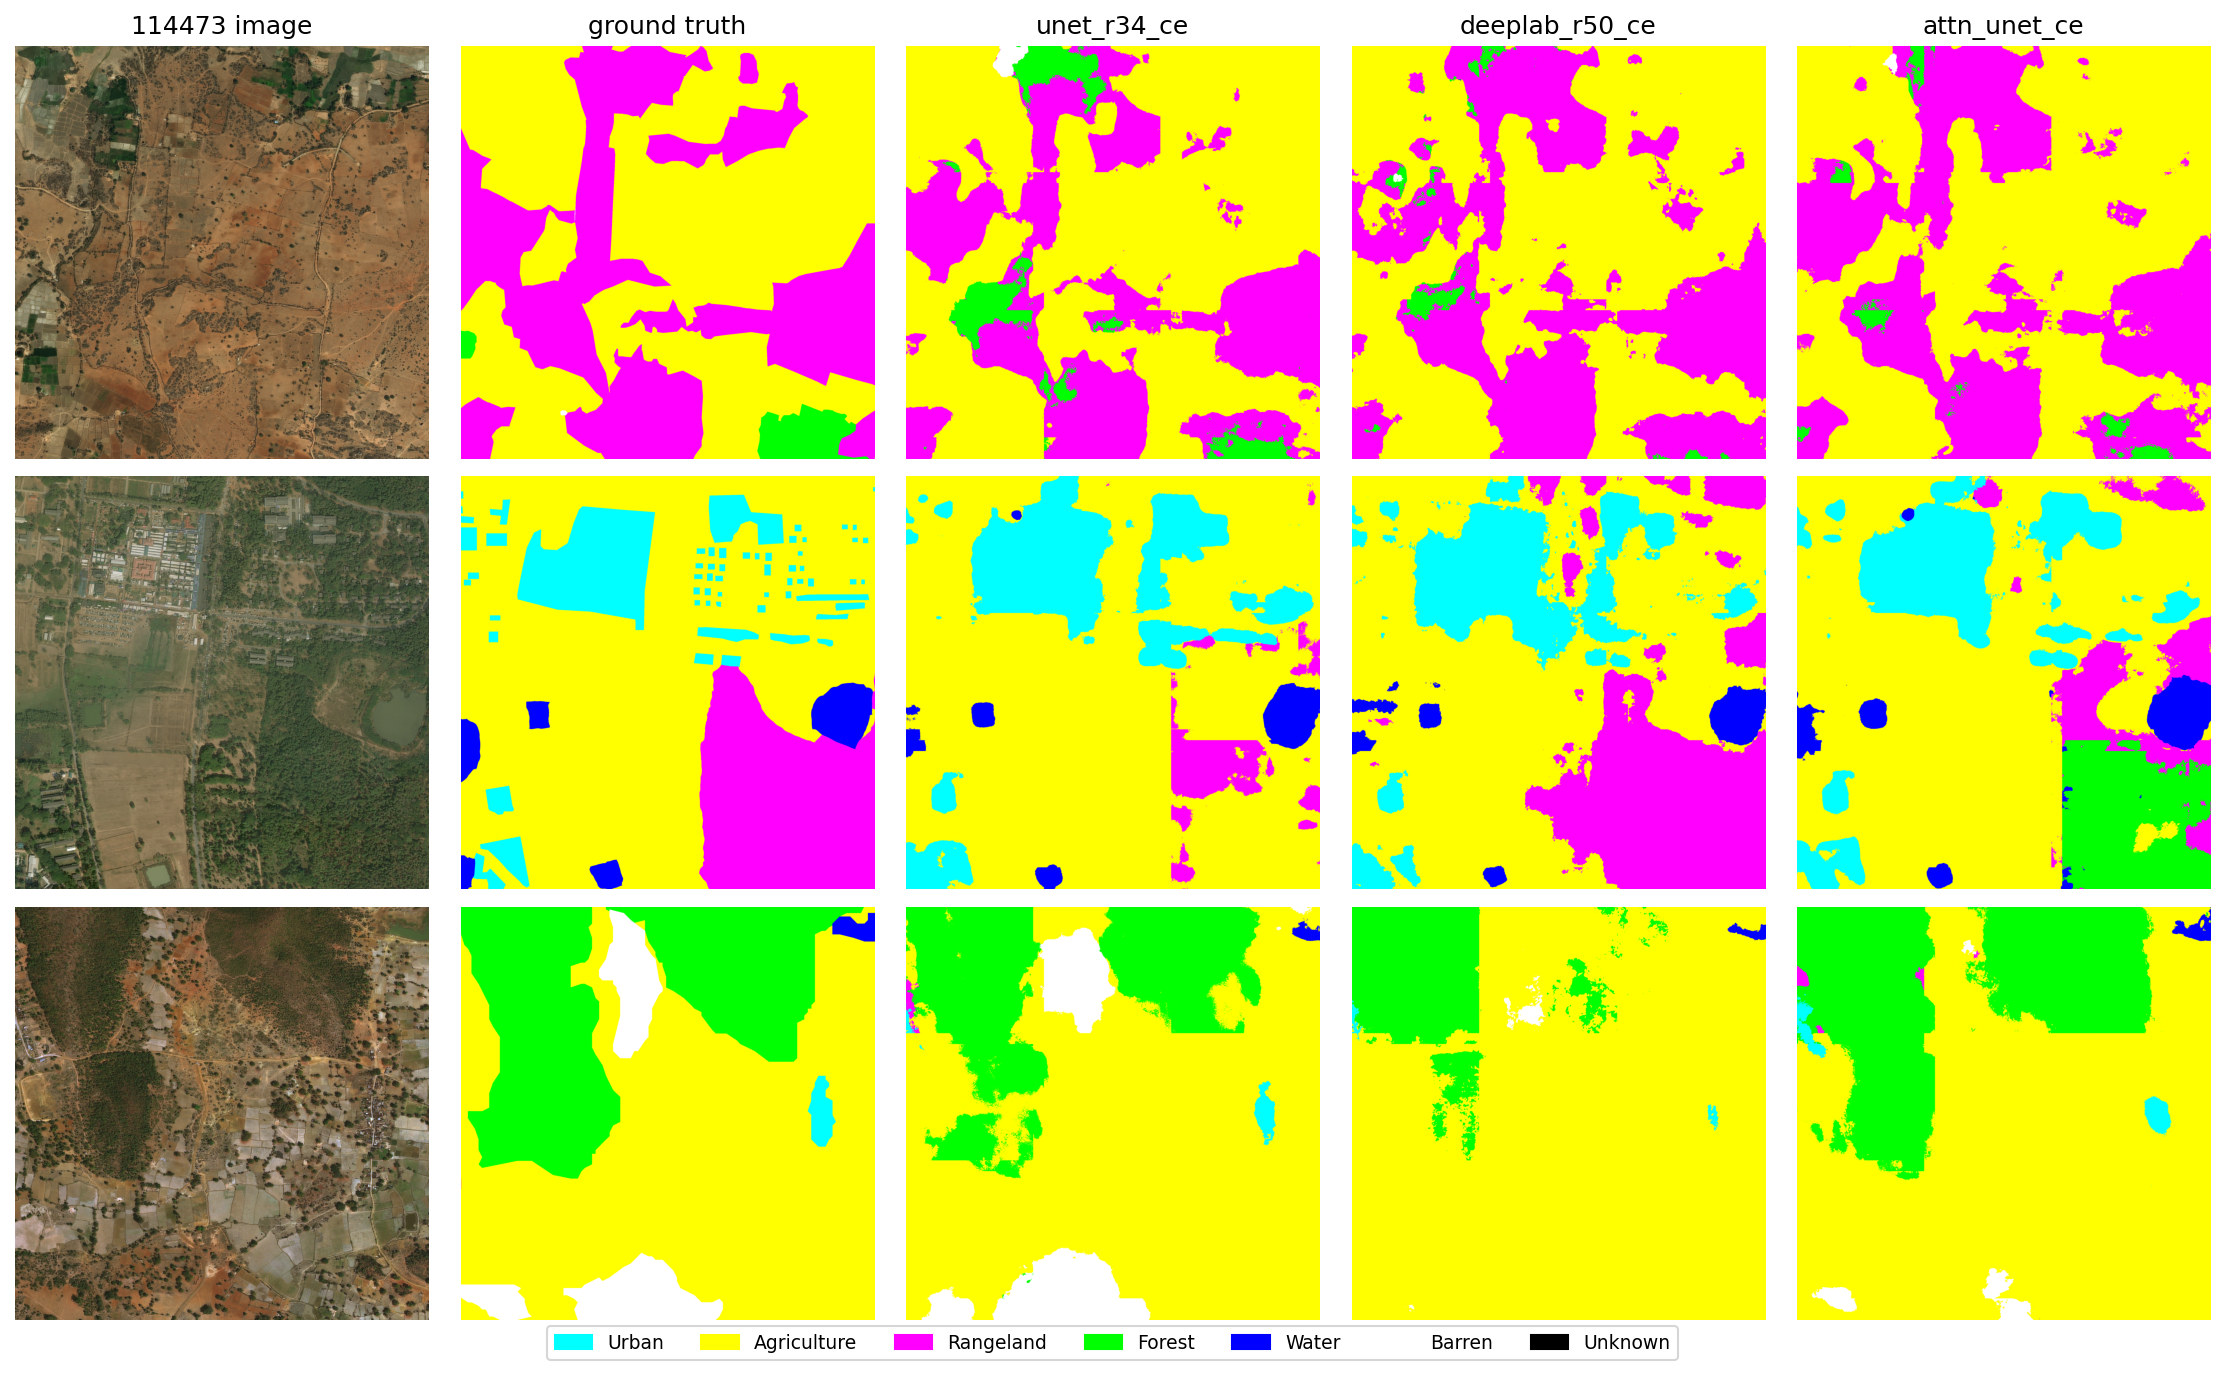
\includegraphics[width=0.95\linewidth]{figs/qualitative.png}

  \vspace{0.2em}
  \scriptsize image \hspace{3em} ground truth \hspace{2em} per-model predictions
\end{frame}

\begin{frame}{Failure cases (DeepLabV3+-R50 + Combined)}
  \centering
  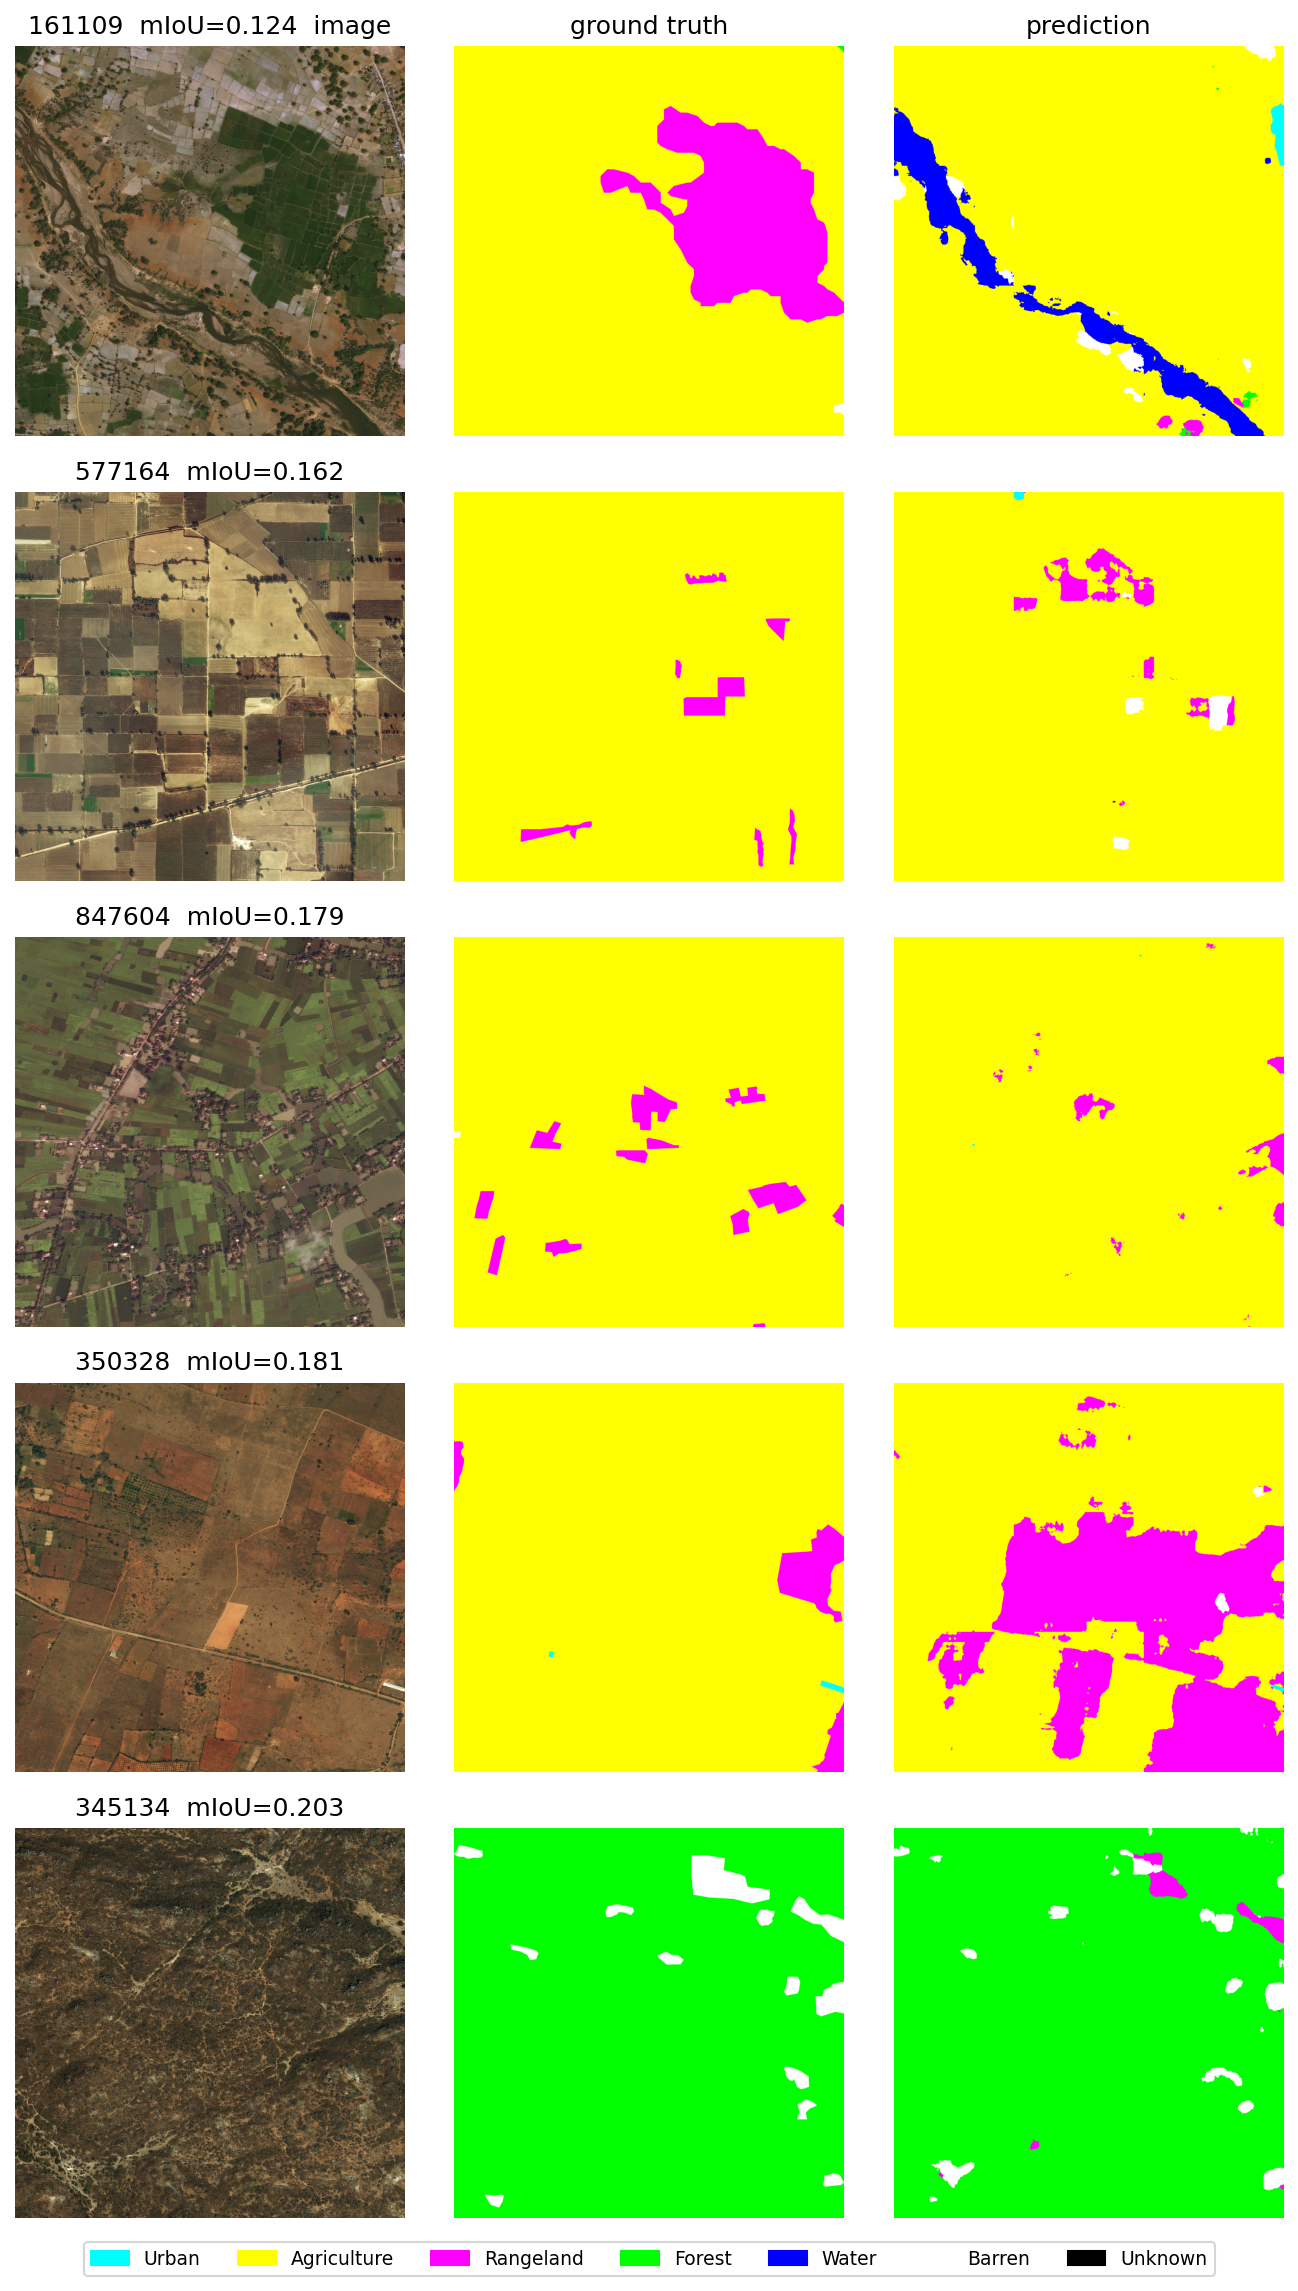
\includegraphics[width=0.9\linewidth]{figs/failures_combined.png}

  \vspace{0.4em}
  \footnotesize
  Errors cluster at semantic boundaries: Rangeland $\to$ Forest,
  urban shadows $\to$ Water, bare agricultural margins $\to$ Barren.
\end{frame}

% ============================================================================
\section{Conclusions}

\begin{frame}{Take-home messages}
  \begin{enumerate}
    \item \textbf{Pre-training} is the biggest single-variable lever:
          $+4.1$ mIoU holding architecture fixed, vs. $\le +1.0$ for any
          single decoder swap among pretrained models. \\
          \textit{Budget pre-training first, architecture second.}
    \item \textbf{Combined CE + Dice} on the same architecture raises
          test mIoU by $+3.7$ and Barren IoU by $+2.0$ over CE alone;
          stacked with the architecture upgrade it yields $+10.5$ Barren
          points vs.\ the Vanilla U-Net baseline. \\
          \textit{Always rebalance the loss for long-tailed segmentation.}
    \item \textbf{Deeper $\neq$ Pareto-optimal}: ResNet101 wins test mIoU
          by only $+0.022$ over R50 while using $71\%$ more parameters
          and $2.4\times$ training time. \\
          \textit{Scale capacity to data, not to the newest paper.}
  \end{enumerate}

  \vspace{0.6em}
  \begin{block}{Best model}
    DeepLabV3+-R50 + Combined loss: \textbf{0.7332 test mIoU} on
    full-resolution reconstructions (120 test images, 7 classes).
  \end{block}
\end{frame}

\begin{frame}{Limitations and future work}
  \begin{itemize}
    \item Single dataset (DeepGlobe)---transfer-learning results may not
          generalize.
    \item No Transformer backbone (Swin, SegFormer) tested.
    \item Class-frequency-weighted loss variants unexplored.
    \item Tile-based inference leaves residual boundary artifacts;
          full-image Transformers could help.
  \end{itemize}

  \vspace{0.8em}
  \textbf{Code, weights, training logs, \& figures}:
  \centerline{\small \url{https://github.com/Jerryzhang258/landcover-seg}}
\end{frame}

\begin{frame}[allowframebreaks]{References}
  \footnotesize
  \begin{thebibliography}{9}
    \setlength{\itemsep}{0.3em}
    \bibitem{demir2018}
      I.~Demir et al.
      \newblock DeepGlobe 2018: A challenge to parse the earth through
      satellite images.
      \newblock \emph{CVPR Workshops}, 2018.

    \bibitem{ronneberger2015}
      O.~Ronneberger, P.~Fischer, T.~Brox.
      \newblock U-Net: Convolutional networks for biomedical image
      segmentation.
      \newblock \emph{MICCAI}, 2015.

    \bibitem{chen2018}
      L.-C.~Chen et al.
      \newblock Encoder--decoder with atrous separable convolution for
      semantic image segmentation (DeepLabV3+).
      \newblock \emph{ECCV}, 2018.

    \bibitem{he2016}
      K.~He et al.
      \newblock Deep residual learning for image recognition (ResNet).
      \newblock \emph{CVPR}, 2016.

    \bibitem{roy2018}
      A.~G.~Roy, N.~Navab, C.~Wachinger.
      \newblock Concurrent spatial and channel squeeze-and-excitation in
      fully convolutional networks (SCSE).
      \newblock \emph{MICCAI}, 2018.

    \bibitem{milletari2016}
      F.~Milletari, N.~Navab, S.-A.~Ahmadi.
      \newblock V-Net and Dice loss for volumetric medical image
      segmentation.
      \newblock \emph{3DV}, 2016.

    \bibitem{lin2017}
      T.-Y.~Lin et al.
      \newblock Focal loss for dense object detection.
      \newblock \emph{ICCV}, 2017.

    \bibitem{iakubovskii2019}
      P.~Iakubovskii.
      \newblock \emph{Segmentation Models PyTorch}.
      \newblock \url{github.com/qubvel/segmentation_models.pytorch}, 2019.

    \bibitem{jadon2020}
      S.~Jadon.
      \newblock A survey of loss functions for semantic segmentation.
      \newblock \emph{IEEE CIBCB}, 2020.
  \end{thebibliography}
\end{frame}

\begin{frame}[standout]
  Thank you.\\
  Questions?
\end{frame}

% ============================================================================
\appendix

\begin{frame}{Backup: Phase 5 per-class IoU}
  \centering
  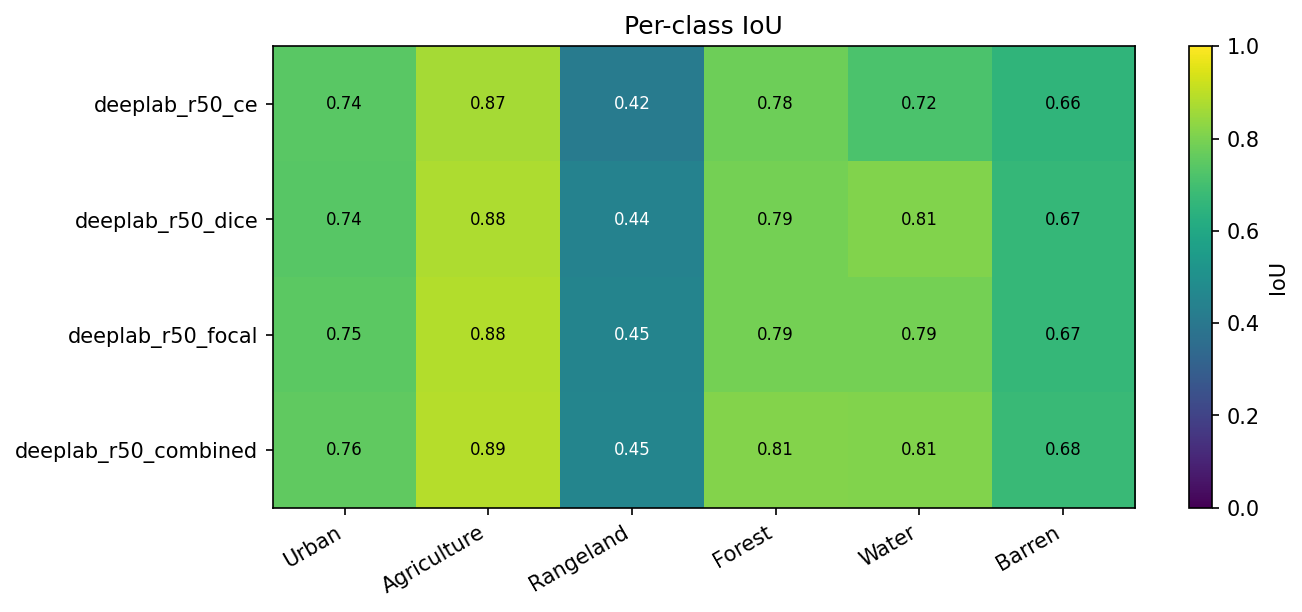
\includegraphics[width=0.8\linewidth]{figs/losses_perclass.png}
\end{frame}

\begin{frame}{Backup: Phase 4 per-class IoU}
  \centering
  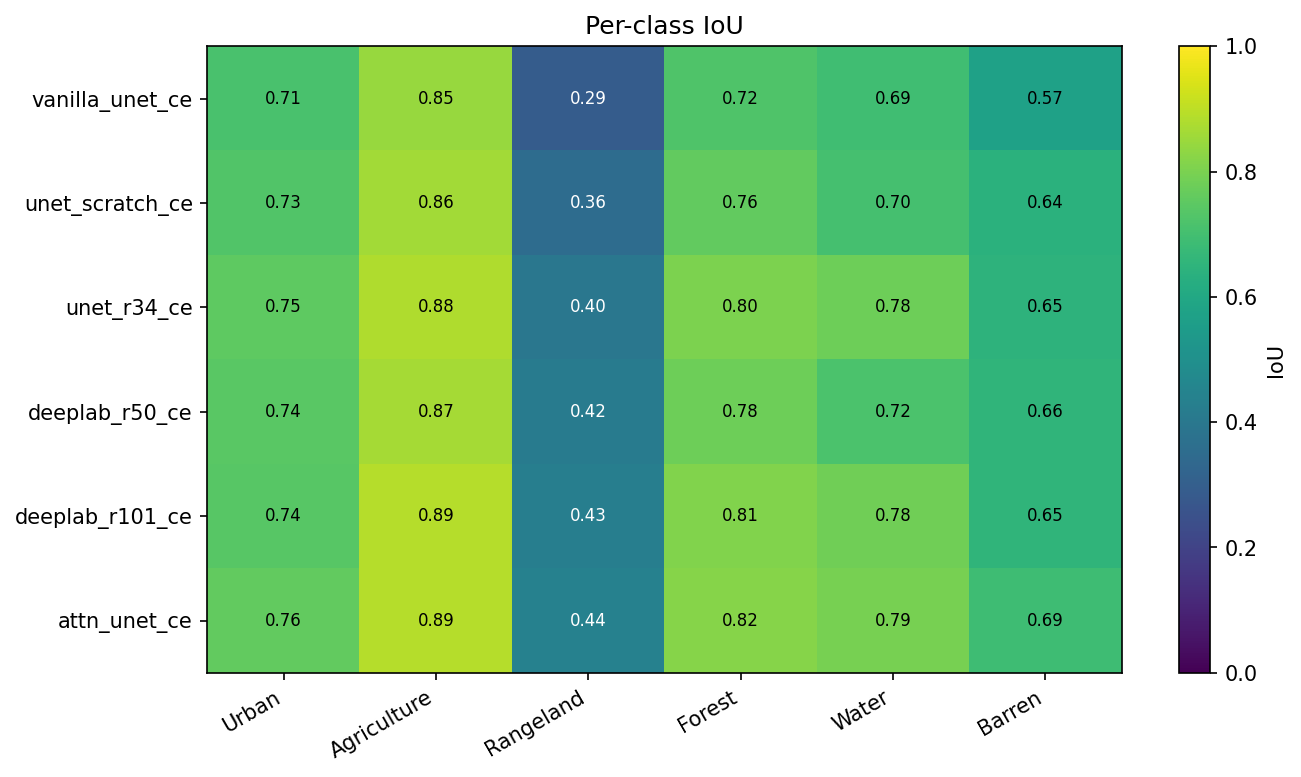
\includegraphics[width=0.8\linewidth]{figs/archs_perclass.png}
\end{frame}

\begin{frame}{Backup: full results table}
  \footnotesize
  \begin{tabular}{l l c c c c c}
  \toprule
  Model & Loss & Params & Val mIoU & Test mIoU & Train (h) & Infer (ms) \\
  \midrule
  vanilla\_unet      & ce       & 31.04 & 0.6442 & 0.6402 & 3.53 & 1046 \\
  unet\_scratch      & ce       & 24.44 & 0.6743 & 0.6750 & 2.00 &  832 \\
  unet\_resnet34     & ce       & 24.44 & 0.7156 & 0.7093 & 1.76 &  799 \\
  deeplab\_r50       & ce       & 26.68 & 0.7201 & 0.6963 & 0.97 &  838 \\
  deeplab\_r101      & ce       & 45.67 & 0.7124 & 0.7178 & 2.32 &  891 \\
  attn\_unet         & ce       & 24.55 & 0.7259 & 0.7316 & 2.20 &  855 \\
  deeplab\_r50       & dice     & 26.68 & 0.7314 & 0.7214 & 2.02 &  821 \\
  deeplab\_r50       & focal    & 26.68 & 0.7286 & 0.7217 & 2.02 &  846 \\
  \rowcolor{accent!15}
  deeplab\_r50       & combined & 26.68 & \textbf{0.7382} & \textbf{0.7332} & 2.02 &  846 \\
  \bottomrule
  \end{tabular}
\end{frame}

\end{document}
